System Architect - Justin

\section{Block Diagram}
\begin{figure}[H]
\centering
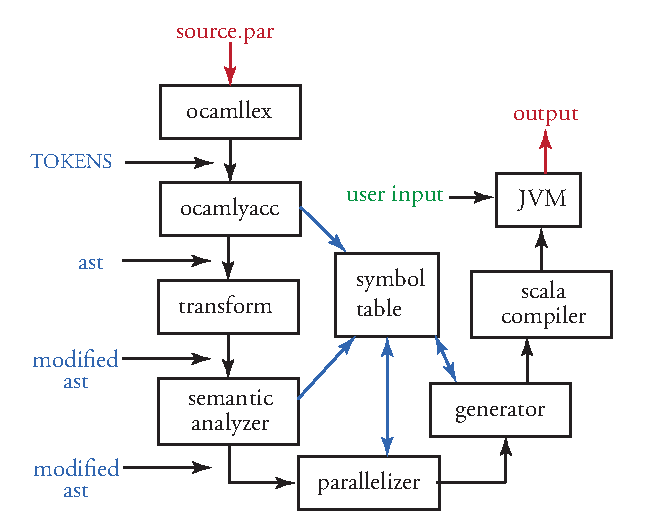
\includegraphics[scale=1]{blockdiagram.eps}
\caption{Caption here}
\end{figure}

\section{Interfaces}
Dotpars interface, as seen above follows a standard form of a
compiler. The raw source file is fed into the lexer, \verb=ocamllex=,
which outputs a series of tokens that is then parsed by the parse,
\verb=ocamlyacc. Ocamlyacc= uses a our type system implemented in the
output a tree like ast with nested types.

Our ast is then undergoes a series of modifications and optimizations
before it is complied down into scala and fed into the scala compiler.
The first transform is done by the aptly named transform which
reverses nodes with a tree.  The lexer recurses right to left, and
thus we need to reverse this.  The transform outputs a modified ast
which is then fed into the semantic analyzer.The semantic analyzer
performs an extensive amount of type checking, making sense of the
source code, throwing errors where need be, fixing things if
necessary, and adding necessary informatino to the symbol table.
Next, the parallelizer, where the main optimizations are done, takes
our modified ast and performs two passes to test what functions, if
any can be parallelized. We focus on major bottlenecks which include
maps, reduces, and list comprehensions. Lastly, the parallelizer
outputs a modified ast which is fed into the generator, which does a
pass over the ast, translating the tree into scala which is then
lastly fed into the scala complier.

\section{Implementation}
The grammar was designed and implemented Sid Nair, and Nathan Hwang,
with the conversion to ocaml being carried out by Sid Nair and Justin
Hines.  The parser was completed by Nathan Hwang and Justin Hines.
The transform by Nathan Hwang.  The Semantic Analyzer was implemented
by Justin Hines and Andrew Hitti.  The Pallelizer was implemented by
Sid Nair, Nathan Hwang, and Justin Hines. The Generator was
implemented by Nathan Hwang with signifcant contributions from Nathan
Hwang, Andrew Hitti and Justin Hines.
